\section{壹、前言}

\subsection{一、研究動機}

近年來,物件追蹤技術被廣泛應用於球類運動上,例如鷹眼系統(Hawk-Eye)已被應用於網球、羽球等運動,以追蹤和記錄球的路徑。然而由於其架設成本高,多數運動員無法負擔。為了解決此問題,國立交通大學網路最佳化實驗室開發了深度學習架構 TrackNet,可以由一般攝影機拍攝之網球比賽影片追蹤網球軌跡。(鍾奉原,2020)

排球在我校是非常興盛的一種運動,經常舉辦班際球賽等排球比賽,因此我們便想利用 TrackNetV2 追蹤排球比賽影片中的排球,以協助分析排球比賽,減少人工花費大量時間觀看的成本。

\subsection{二、研究目的}

應用 TrackNetV2 追蹤由一般攝影機(非高速攝影機)所錄製之排球比賽影片中的排球,藉由自動追蹤球的路徑協助排球比賽的賽事分析。

\subsection{三、文獻回顧}

傳統影像物件辨識是根據物件的外顯特徵和統計特徵進行偵測的,但排球比賽中的排球會因打擊的關係而導致有變形的情況出現,再加上移動速度過快,快門相對於球的速度來說較慢,因此容易有影像殘留及模糊的現象出現。

\begin{itemize}
    \setlength\parindent{2em}
    \item []
    \textbf{(一)TrackNet}

    TrackNet(黃昱銓,2018)提出了一個以 CNN(Convolutional Neural Network,卷積神經網路)為基礎的深度學習架構(如圖 \ref{TrackNet 架構圖})。但不同於其他深度學習網路,它容許一次輸入多張連續幀,可從中學習球的影像特徵及軌跡特性。然後仿效 FCN(Fully Convolutional Network,全卷積網路)的生成階段,生成用於偵測及定位球的熱度圖(如圖 \ref{熱度圖})。最後再依據熱度圖計算畫面中可能存在的網球。這個模型不僅能從模糊影像中定位球的存在,更可以進一步的判斷受遮擋的網球位置,可以很好的達到我們的需求。
    
    \begin{figure}[H]
        \centering
        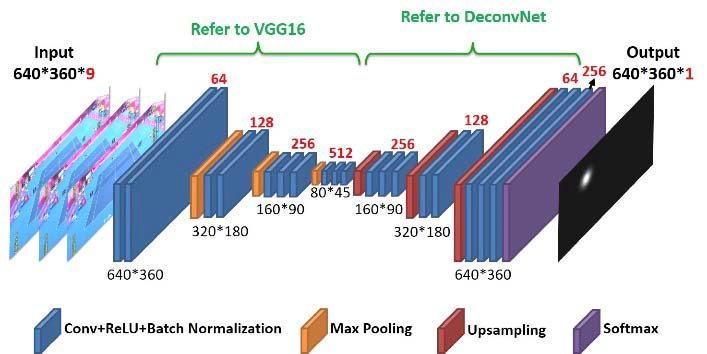
\includegraphics[width = 9cm]{picture/TrackNet 架構圖.jpg}\\
        \caption{、TrackNet 架構圖(黃昱銓,2018)}
        \label{TrackNet 架構圖}
        \vspace{1cm}
        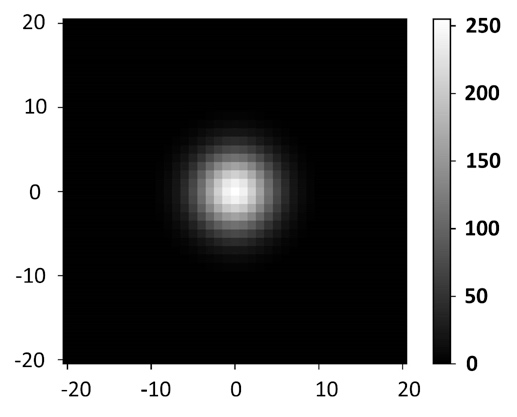
\includegraphics[width = 7cm]{picture/熱度圖.jpg}
        \caption{、熱度圖(黃昱銓,2018)}
        \label{熱度圖}
    \end{figure}
    \item[]
    \textbf{(二)TrackNetV2}

    TrackNetV2(Nian-En Sun et al., 2020)在 TrackNet 的基礎上改進了它的處理速度、準確度、記憶體用量等。他們將 TrackNet 的模型重新設計,讓它從一個 MISO(Multiple-In Single-Out)的模型變成一個 MIMO(Multiple-In Multiple-Out)的模型,處理速度從原本的 2.6 FPS(Frame per second)上升到 31.8 FPS。他們也參考了 U-Net 的 skip connection(殘差連接),將卷積層所得的特徵圖(feature map)串聯到相應的上採樣層(upsampling layer),以此方式將低層次與高層次的特徵結合起來以提高準確度。他們所使用的資料集為來自 18 場羽球比賽共 55563 幀的羽球比賽影片。

    \begin{figure}[H]
        \centering
        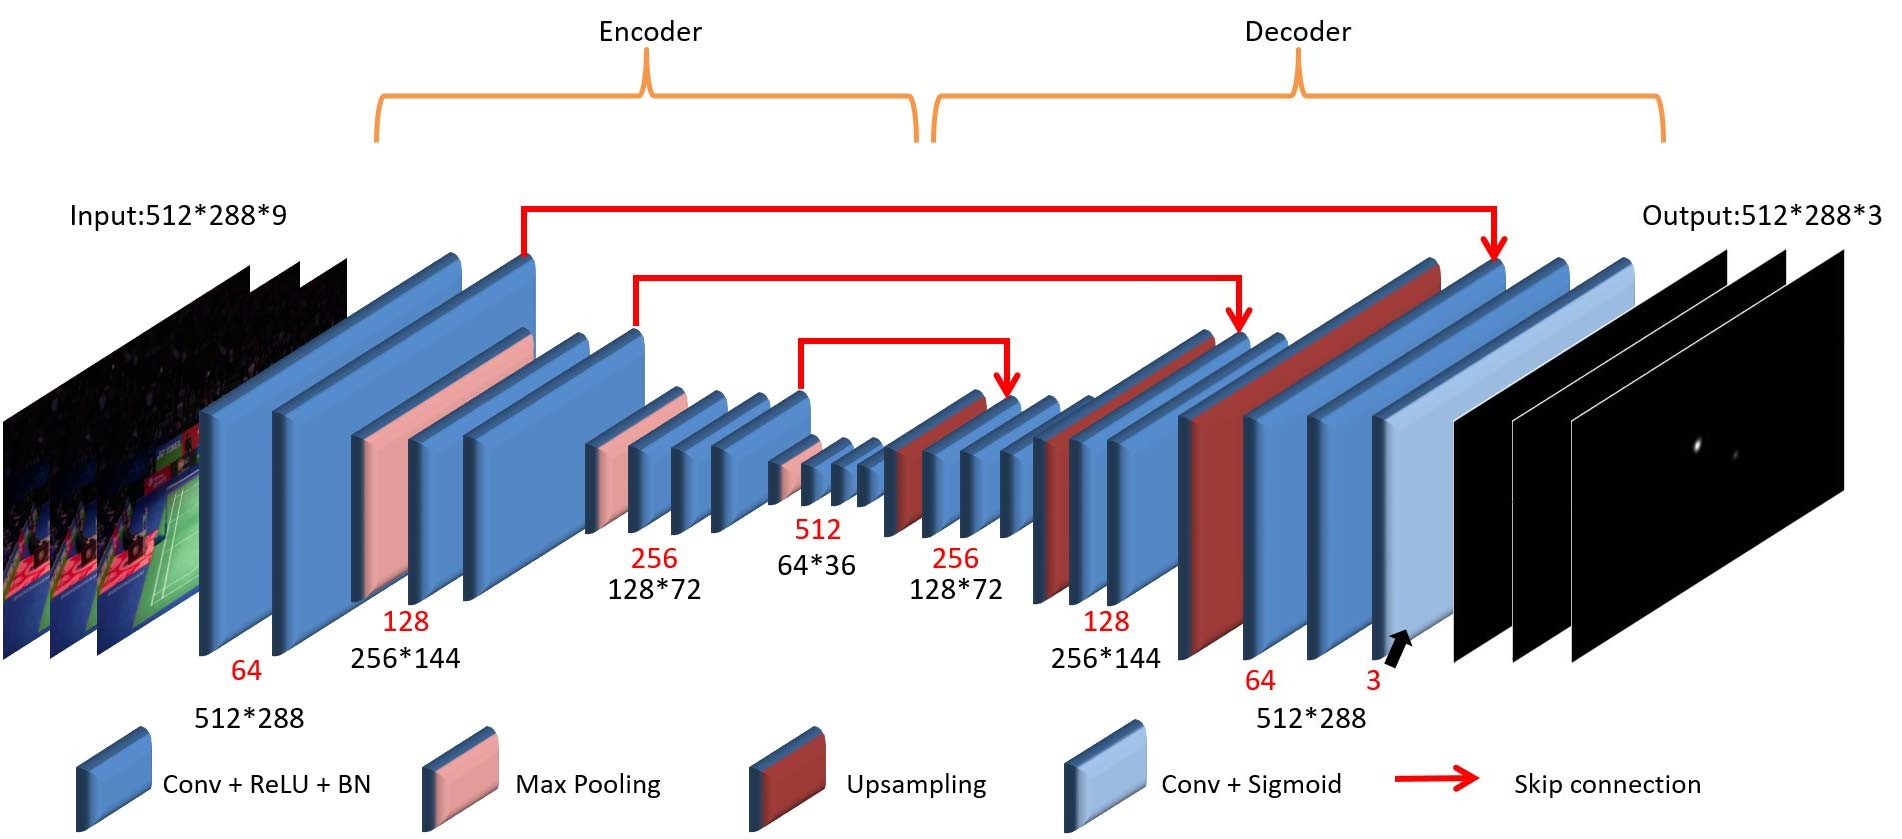
\includegraphics[width = 9cm]{picture/TrackNetV2 架構圖.jpg}
        \caption{、TrackNetV2 架構圖(Nian-En Sun et al., 2020)}
        \label{TrackNetV2 架構圖}
    \end{figure}

    \item[]
    \textbf{(三)卷積神經網路}

    卷積神經網路(Convolutional Neural Network, CNN)是一種深度學習的神經網路模型,常被應用於影像識別方面。CNN 的結構包含卷積層(Convolution Layer)、池化層(Pooling Layer)、全連接層(Fully Connected Layer)。

    \begin{itemize}
        \setlength\parindent{2em}
        \item []
        \textbf{1. 概念}

        \begin{itemize}
            \setlength\parindent{2em}
            \item []
            \textbf{(1)權值共享}

            在一般的圖像內有許多的特徵是相同的,如特定的輪廓或線條,那我們就可以讓相同幾個神經元組成的卷積核去學習這個特徵,透過滑動窗口對整張圖片進行卷積,進而達到節省參數的效果。(Cinnamon AI Taiwan,2019)

            \item[]
            \textbf{(2)保留位置資訊}

            圖片中的像素(Pixels)與其鄰近的像素會有一定的關聯度,若使用 FC(Fully Connected,全連接網路結構)的結構來訓練圖像資訊的話,要先通過一個展開(Flatten)的步驟,把高維的資訊拉成一條直線,如此一來就會大量失去特徵之間的空間資訊。(Cinnamon AI Taiwan,2019)
        \end{itemize}

        \item[]
        \textbf{2. 結構}

        \begin{itemize}
            \setlength\parindent{2em}
            \item []
            \textbf{(1)卷積層(Convolution Layer)}

            卷積層負責提取圖像中的局部特徵,其原理是透過許多的卷積核(kernel)在圖片上進行滑動擷取特徵。將圖片與特定的卷積核進行卷積運算。

            \begin{figure}[H]
                \centering
                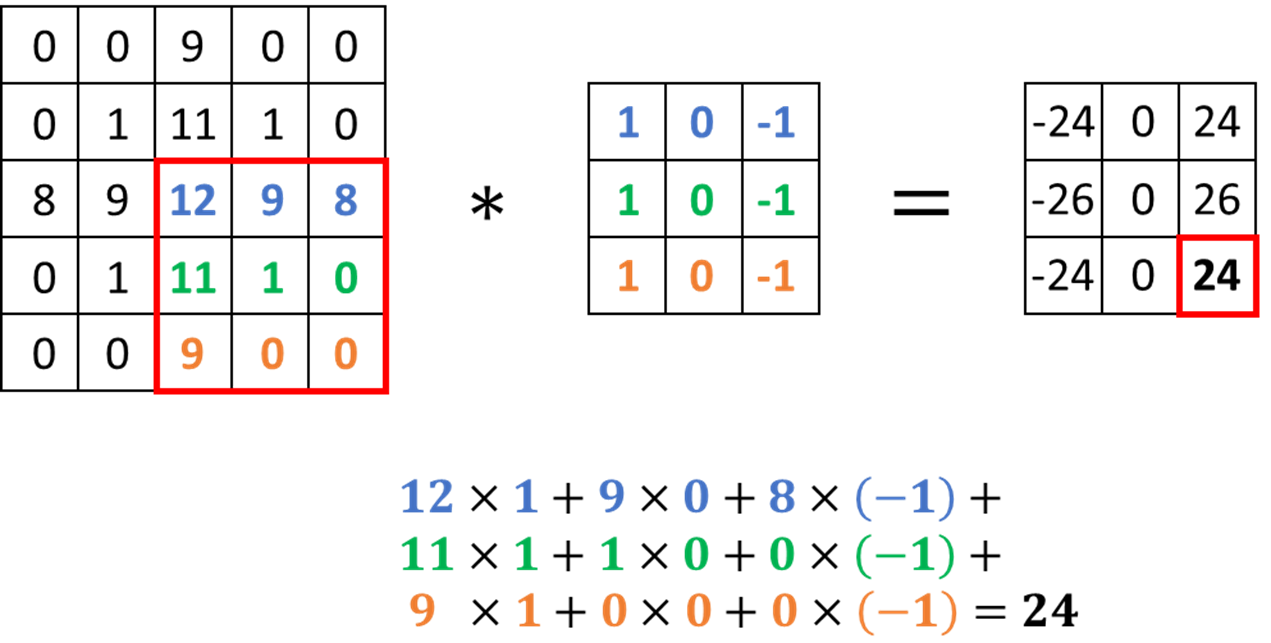
\includegraphics[width = 9cm]{picture/卷積層.jpg}
                \caption{、卷積層(Brandon Da Silva,2018)}
                \label{卷積層}
            \end{figure}

            \item[]
            \textbf{(2)池化層(Pooling Layer)}

            池化層是用來大幅降低參數量級(降維)、降低過擬合問題、緩解卷積層對位置的敏感度。池化層的計算與卷積層一樣,都是透過滑動視窗框選的局部數值進行數值運算,最常用的計算方式為 Max pooling,在框選的局部數值中挑出最大值。(李謦伊,2020)
        
            \begin{figure}[H]
                \centering
                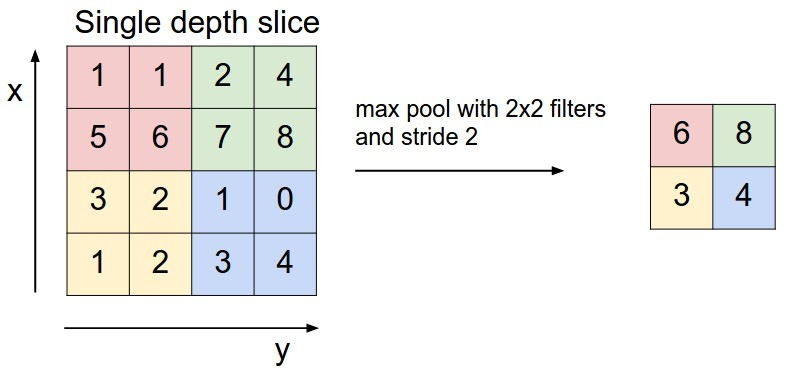
\includegraphics[width = 9cm]{picture/池化層.jpg}
                \caption{、池化層(Max pooling)(cs231n,2021)}
                \label{池化層}
            \end{figure}

            \item[]
            \textbf{(3)全連接層(Fully Connected Layer)}

            在經過攤平(Flatten)變為一維數據後,全連接層(FC)主要在做最後的特徵提取,並且利用最後一層 FC 當作分類器。

        \end{itemize}
    \end{itemize}
\end{itemize}

\section{貳、研究設備與器材}

\subsection{一、硬體設備}

\begin{itemize}
    \item [](一)中央處理器(CPU) AMD Ryzen 9 5950X 16-Core Processor
    \item [](二)記憶體:32GiB
    \item [](三)圖形處理器 (GPU):NVIDIA GeForce RTX 3090 (GPU 記憶體 24 GiB)
    \item [](四)作業系統:Linux (Ubuntu 20.04.01)
\end{itemize}

\subsection{二、軟體及工具環境}

\begin{itemize}
    \item [](一)Python 3.7.13:具有高效能的高階資料結構,直譯式且物件導向的程式語言。
    \item [](二)moviepy.editor 1.0.3:是一個 Python 用來編輯影片的函式庫。
    \item [](三)PyQt5 5.15.7:是一個 Python 用來創建圖形使用介面(Graphical User Interface, GUI)應用程式的函式庫。
    \item [](四)pandas 1.3.5:是一個 Python 用來操作及分析資料的函式庫。
    \item [](五) PyMySQL 1.0.2:是 Python 用來連接到 MySQL 資料庫伺服器的一個介面。
    \item [](六)opencv-python 4.6.0.66:是一個用於解決電腦視覺相關問題的 Python 函式庫。
    \item [](七)imutils 0.5.4:整合了 OpenCV 、 numpy 和 matplotlib 的相關操作的套件,主要用於進行圖像處理。
    \item [](八)Pillow 9.2.0:是一個 Python 中用於影像辨識的套件庫,可以用來旋轉照片、嵌字、合成照片、變更圖片解析度等。
    \item [](九)piexif 1.1.3:可以讀取與修改圖片 Exif(可交換圖檔格式)的套件,通常與 Pillow 搭配使用。
    \item [](十)scikit-learn 1.0.2:是一個開源資料分析函式庫,具有各種分類、回歸和集群分析。
    \item [](十一)keras 2.9.0:是一款用 Python 編寫而成的開源神經網路函式庫,能搭配 TensorFlow 、 Theano 等運作。
    \item [](十二)TensorFlow 2.9.2:是現在重要的深度學習框架之一,支援各式不同的深度學習演算法。
    \item [](十三)CUDA 10.1.243:是用於圖形處理單元(graphical processing units,GPU)的平行運算平台和程式設計模型。
\end{itemize}

\section{參、研究過程或方法}

\section{肆、研究結果}

\section{伍、討論}

\section{陸、結論}

\section{柒、參考文獻資料}
\begin{itemize}
    \item [一、] 10 程式中(2021 年10 月6 日)。[Day 24] 機器學習- 不能忽視的過擬合與欠擬
    合。檢自:\url{https://ithelp.ithome.com.tw/articles/10278254}
\end{itemize}